\documentclass[11pt]{article}
%Gummi|061|=)
\title{\textbf{Characteristics}}
\author{Nicolas}
\date{}
\usepackage{graphicx}
\usepackage{amsmath}
\usepackage[left=2cm,right=2cm,top=2cm,bottom=2cm]{geometry}
\newcommand{\p}[2]{\ensuremath{\frac{\partial {#1}}{\partial {#2}}}}
\newcommand{\hphi}{\ensuremath{\hat{\phi}}}

\begin{document}

\maketitle

\section{Goal and idea}
We want to solve the segregation equation
\begin{equation} \label{eq:conservative_form}
	\p{\phi}{t} + \p{u\phi}{x} + \p{v\phi}{y} + \p{w\phi}{z} - \p{\phi(1-\phi)}{z} = 0
\end{equation}

We are looking for a steady-state solution in the frame travelling at the (constant) speed of the front $u_F$. So by making the change of variable $ x \leftarrow x - u_F t$ we are left with

\begin{equation}
	\p{u\phi}{x} + \p{v\phi}{y} + \p{w\phi}{z} - \p{\phi(1-\phi)}{z} = 0
\end{equation}
We can make use of incompressibility, to take the velocity components out of the partial derivatives:
\begin{equation}
	u\p{\phi}{x} + v\p{\phi}{y} + w\p{\phi}{z} - \p{\phi(1-\phi)}{z} = 0
\end{equation}
and since $v = 0$ in the centre plane, we have
\begin{equation} \label{eq:segreg}
	u\p{\phi}{x} + w\p{\phi}{z} - \p{\phi(1-\phi)}{z} = 0
\end{equation}

Our goal is to find a solution of this equation. 
This is not an easy problem, because \cite{eq:segreg} is a \textit{partial derivatives equation}, and we have very few tools at our disposal to solve exactly this kind of differential equations.
Two things will help us. 
First, this equation can be seen as a \textit{conservation law}. Indeed if we call $\mathbf{\hat{u}}$ the velocity field 
\begin{equation}
	\mathbf{\hat{u}} = 
	\begin{pmatrix}
	u\\
	v\\
	w - (1 -\phi)\\
	\end{pmatrix}
\end{equation}
we can rewrite \cite{eq:conservative_form} as
\begin{equation}
	\p{\phi}{t} + \mathbf{\nabla} \cdot (\mathbf{\hat{u}} \phi) = 0
\end{equation}
Now we can see that the concentration in small particles,  $\phi$ is a \textit{conserved quantity} for which the flux is $\mathbf{\hat{u}} \phi$. In other words, small particles are advected without diffusion at speed $\mathbf{\hat{u}}$. 
Conservation laws can be solved using the \textit{method of the characteristics}.

\subsection{Method of the characteristics}
We can rewrite \cite{eq:segreg} as 
\begin{equation} \label{eq:carac_form}
		u\p{\phi}{x} + w\p{\phi}{z} - (1 - 2\phi)\p{\phi}{z} = 0
\end{equation}
The steady-state solution is a function of 2 variables: $ \phi = \phi(x, z)$. So the solution can be seen as the surface $ \phi - \phi(x,z) = 0$ of the 3D space $(x, z, \phi)$. 
Characteristics are curves $\phi = \hphi(x(s),z(s))$ lying on this surface, and verifying
\begin{equation}
	\frac{d \hphi}{d s} = 0
\end{equation}
Using chain rule we have 
\begin{equation}
	\p{x}{s} \p{\hphi}{x} + 
	\p{z}{s}\p{\hphi}{z} = 0
\end{equation} 
and since $\hphi$ is lying on the solution surface,
\begin{flalign}
\p{x}{s} = u \\
\p{z}{s} = w - (1- 2 \phi)
\end{flalign}
Secondly, conservation laws can easily be solved numerically with great accuracy. Solving numerically the problem gives us a useful insight (\cite{fig:1}).
\begin{figure}[htp]
\centering
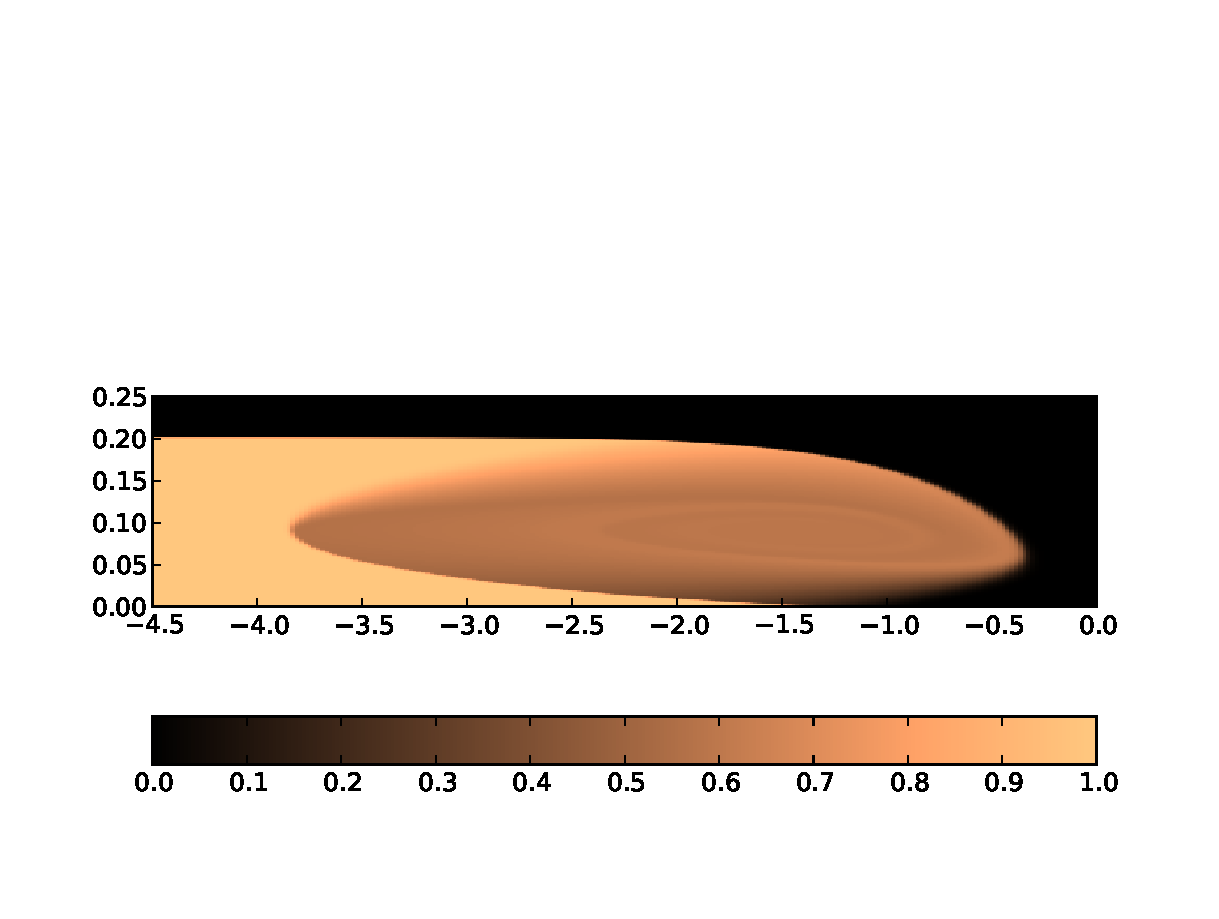
\includegraphics[scale=0.70]{spiral.pdf}
\caption{From the numerically computed steady-state solution we can deduce the general structure of the steady-state.}
\label{fig:1}
\end{figure}


\end{document}